\documentclass[12pt,a4paper]{beamer}
\usepackage{graphicx}
\usepackage{hyperref}
\usepackage{lmodern}
\usepackage{listings}
\usepackage[utf8x]{inputenc}
\usepackage[L7x]{fontenc}
\usepackage[lithuanian]{babel}
\usepackage{minted}

% Theme
\usetheme{Antibes} 
\usecolortheme[RGB={155,192,12}]{structure} 

\definecolor{codebg}{rgb}{0.10, 0.11, 0.08}
\definecolor{bashbg}{rgb}{0.95,0.95,0.95}
\definecolor{xmlbg}{rgb}{0.20, 0.22, 0.18}

% Code highlight setup
\usemintedstyle{monokai}
\newminted{c}{
    linenos,
    bgcolor=codebg,
    fontsize=\scriptsize,
    gobble=4
}

\author{Povilas Balzaravičius}
\title{Augalų monitoringas su Arduino}
\subtitle{No Trolls Allowed 2013}

\begin{document}
\section{Įžanga}
\begin{frame}
	\titlepage
\end{frame}

\begin{frame}{Kas aš toks?}
    \begin{itemize}
        \item Povilas Balzaravičius
        \item \href{https://twitter.com/pawka}{@Pawka}
        \item \href{https://github.com/pawka}{github.com/pawka}
        \item \href{https://linkedin.com/in/pawka}{linkedin.com/in/pawka}
        \item \href{http://pawka.linija.net}{pawka.linija.net}
    \end{itemize}
    \begin{center}
        
\includegraphics[scale=0.4]{img/estina.png}
        \hskip1.5cm
        
\includegraphics[scale=0.4]{img/zce.png}
        \hskip1.5cm
        
\includegraphics[scale=0.75]{img/ktu.png}
    \end{center}
\end{frame}

\begin{frame}
    \frametitle{Analog - įdomu!}

    \begin{center}
        Programuotojams įdomu kontroliuoti analoginius dalykus.
    \end{center}
    \pause
    \begin{center}
        {\Huge Išeitis - Arduino!}
    \end{center}

\end{frame}

\begin{frame}
    \frametitle{Arduino}

    \begin{itemize}
        \item Mikrokontroleris
        \item 16 Mhz CPU
        \item 0.5 Kb EEPROM
        \item 3.3-5V
        \item C-stiliaus kalba
    \end{itemize}
    
\end{frame}

\begin{frame}
    \frametitle{Patirtis}
	\begin{center}
        {\Huge NULL}
	\end{center}
    \begin{center}
        (nesuprantu elektros)
    \end{center}
\end{frame}


\begin{frame}[fragile]{Kaip veikia?}
\begin{ccode}
    void setup() {                
        pinMode(OUPTUT_LED_PIN, OUTPUT);
        pinMode(MOISTURE_LED_PIN, OUTPUT);
        Serial.begin(9600);
    }

    void loop() {
        //Logika...
    }
\end{ccode}
\end{frame}

\begin{frame}
    \frametitle{Ką esu nuveikęs?}

    \pause
    \begin{itemize}
        \item Mirksintį LED'ą :-|
        \pause
        \item Termometrą (dafuq?)
        \pause
        \item Prijungęs LED matricą (???)
        \pause
        \item Sąsają NAS'ui. (atsibodo)
    \end{itemize}
    \pause
    \begin{center}
        NUOBODU!
    \end{center}
\end{frame}

\begin{frame}
    \frametitle{Svajonių projektas}

    \begin{center}
        {\Huge Garden Bot*}
    \end{center}

    \vskip1cm
    {\small *Įtakotas uošvienės.}
    
\end{frame}

\begin{frame}
    \frametitle{Ką daro svajonių projektas?}

    \begin{itemize}
        \item Stebi mikroklimatą
        \item Renka statistiką
        \item Laisto šiltnamį
        \item Atidarinėja langus
        \item Nuperka alaus
    \end{itemize}
\end{frame}

\begin{frame}
    \frametitle{Ką dabar daro svajonių projektas?}

    \begin{itemize}
        \item Matuoja drėgmę
        \item Matuoja temperatūrą
        \item Matuoja šviesą
        \item Uždega LED'ą kai trūksta vandens :-)
    \end{itemize}
    
\end{frame}

\begin{frame}
    \frametitle{Schema}
    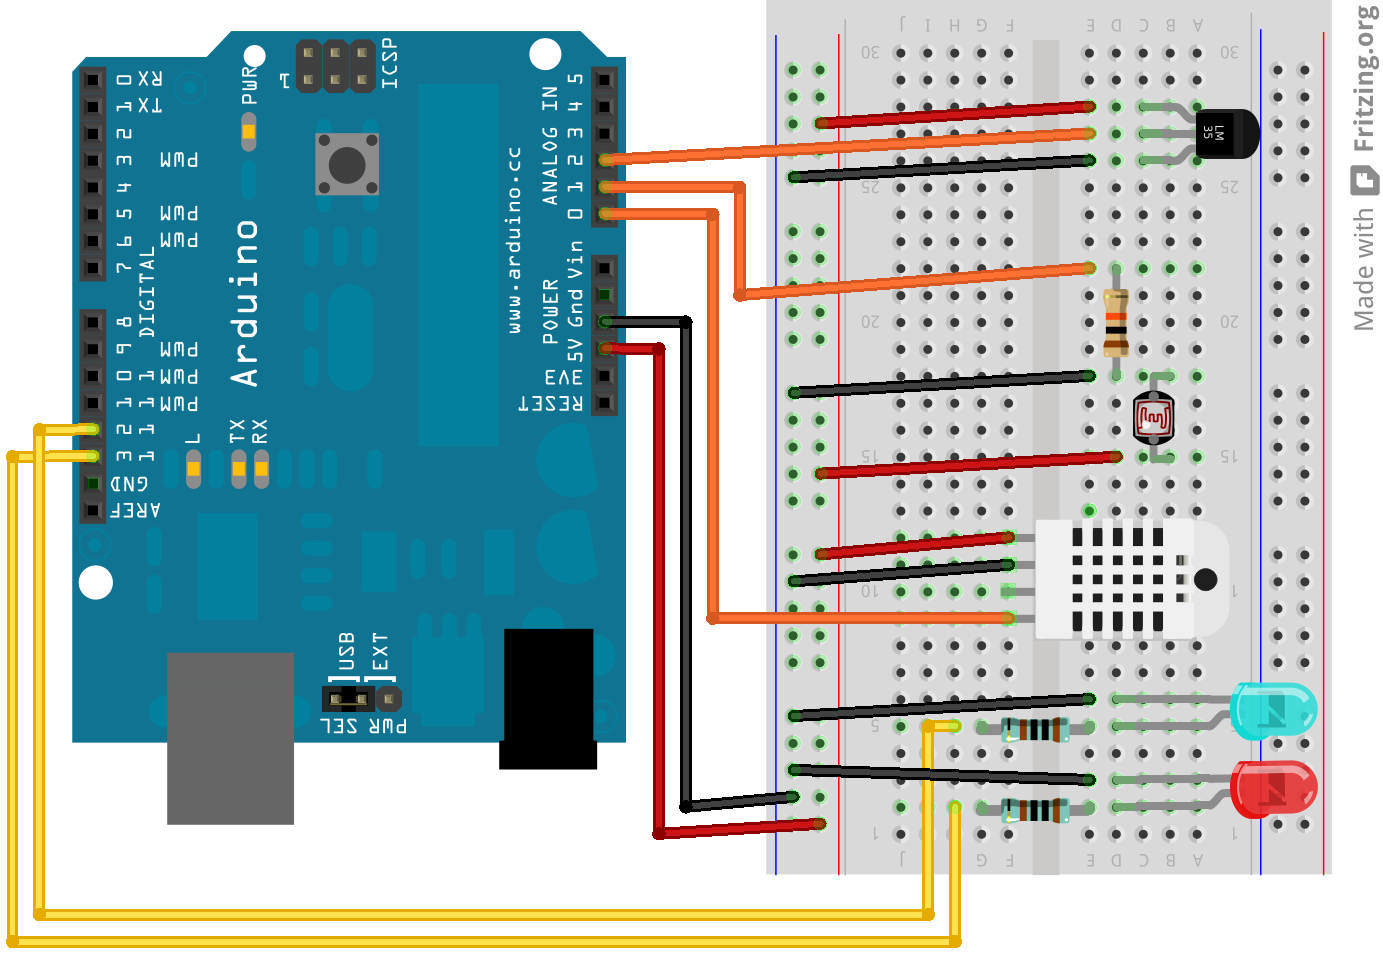
\includegraphics[scale=0.2]{img/schema.png}
\end{frame}

\begin{frame}
    \frametitle{Duomenų perdavimas}

    Duomenys siunčiami per USB. Klauso python skriptas.\\
    \vskip1cm
    Protokolas: XXX;INFO

    \begin{itemize}
        \item XXX - komandos prefix'as.
        \item INFO - Reikšmės/informacija (neprivaloma)
    \end{itemize}
\end{frame}

\begin{frame}
    \frametitle{Komandos}
    
    IN (į kontrolerį):
    \begin{itemize}
        \item NFO - Išplėstinė informacija.
        \item MOI;XX - Nustatyti drėgnumo ribą.
        \item TIM;XX - Nustatyti duomenų siuntimo periodą sekundėmis.
    \end{itemize}

    OUT:
    \begin{itemize}
        \item DAT;MOISTURE;LIGHT;TEMPERATURE
    \end{itemize}

\end{frame}

\begin{frame}
    \frametitle{Kodėl įdomu?}
    Web programuotojui retai sutinkamos problemos.
    \vskip1cm
    \begin{itemize}
        \item EEPROM vienu adresu saugoma maksimali reikšmė - 255. Kaip saugot didesnes reikšmes?
        \item Kaip neblokuoti centrinio ciklo? 
        \item Kaip sutilpti (atminties atžvilgiu)?
        \item Kaip minimizuoti jungčių naudojimą?
    \end{itemize}
    
\end{frame}

\begin{frame}
    \frametitle{Statistika}

    \begin{center}
        Vakar perkeldamas filmą suformatavau flash'ą su duomenim :-(
    \end{center}

    \pause
    Kiek pamenu\ldots
    \begin{itemize}
        \item Naktį drėgmės kritimas minimalus.
        \item Kiek prilaistau, mano buto sąlygomis išgaruoja per 3 dienas.
        \item Šviesos kreivėje matosi kada einu miegot (įjungiama/išjungiama šviesa) :-)
    \end{itemize}

\end{frame}

\begin{frame}
    \frametitle{Ateitis}

    \begin{itemize}
        \item StatsD + Graphite naudojimas duomenų monitoringui (nespėjau).
        \item Duomenų siuntimas/gavimas per WiFi (Xbee modulis).
        \item Daugiau analoginių veiksmų (langų atidarymas, laistymas). Pritaikymas šiltnamiui.
        \item Daugiau konfigūracijos aukščiau aprašytiems veiksmams.
    \end{itemize}
    
\end{frame}

\section{Pabaiga}

\subsection{Išvados}
\begin{frame}{Išvados}
    \begin{itemize}
        \item Arduino - super paprasta.
        \item Neperkelinėti filmų išgėrus alaus.
    \end{itemize}
\end{frame}

\begin{frame}
	\begin{center}
        {\Huge Ačiū}
	\end{center}
\end{frame}

\end{document}
